\chapter{Unifying Machine Learning and Quantum Mechanics} \label{chp:VMCwRBM}
%\epigraph{Great quote.}{Author}
\iffalse
\begin{figure}[H]
	\centering
	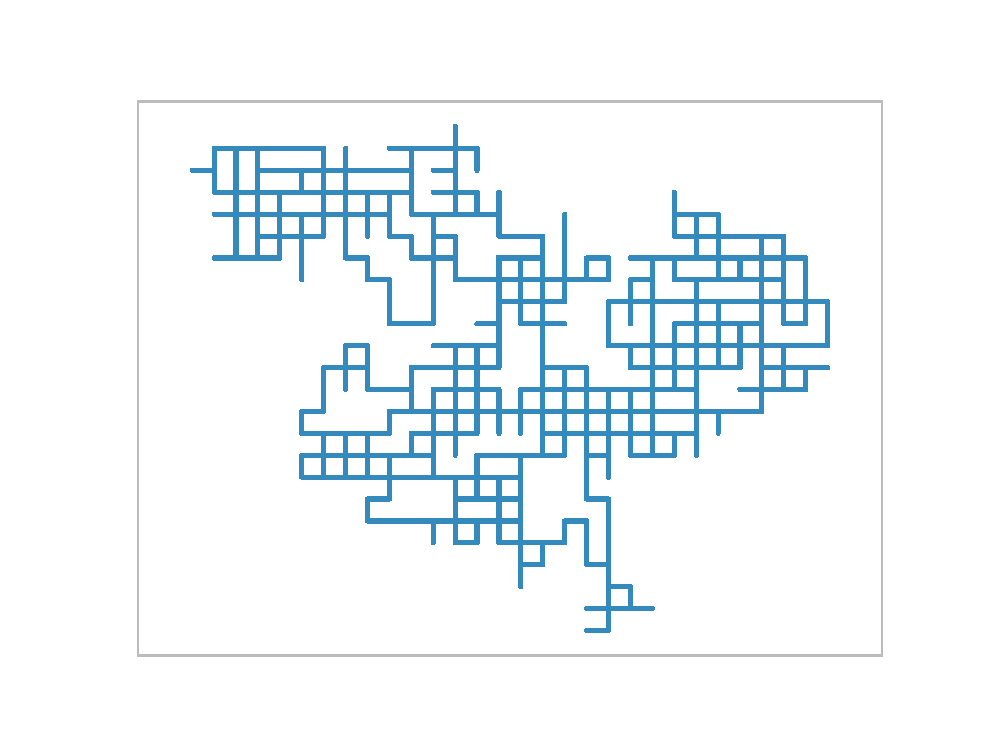
\includegraphics[scale=0.6]{../Images/randomwalk.eps}
	\caption{Random walker on a two-dimensional grid, 1000 moves.}
\end{figure}
\fi

Now as we have introduced the necessary theory, both in the form of quantum theory and machine learning theory, in addition to detailing the variational Monte Carlo (VMC) method, we are ready to unify the machine learning and quantum mechanics. As hinted above, the way we do this is to 

\section{The wave function ansatz} \label{sec:ansatz}
Flexible wave function is needed, with as little physical intuition as possible. However, as mentioned before, the wave function needs to obey Fermi-Dirac statistics, which is done by using the Slater determinant,
\begin{equation}
\Psi_T(\bs{R})\propto
\begin{vmatrix}
\psi_1(\boldsymbol{r}_1,\sigma_1) & \psi_2(\boldsymbol{r}_1,\sigma_2) & \hdots & \psi_N(\boldsymbol{r}_1,\sigma_N)\\
\psi_1(\boldsymbol{r}_2,\sigma_1) & \psi_2(\boldsymbol{r}_2,\sigma_2) & \hdots & \psi_N(\boldsymbol{r}_2,\sigma_N)\\
\vdots & \vdots & \ddots & \vdots \\
\psi_1(\boldsymbol{r}_N,\sigma_1) & \psi_2(\boldsymbol{r}_N,\sigma_2) & \hdots & \psi_N(\boldsymbol{r}_N,\sigma_N)
\end{vmatrix}
\end{equation}
like in standard variational Monte Carlo (VMC). Unlike in standard VMC, the single-particle wave functions $\phi(\bs{r},\sigma)$ will be chosen by a restricted Boltzmann machine, more specific they will be the marginal distribution of the visible units,
\begin{equation}
\psi(\bs{r})=P(\bs{r}).
\end{equation}

\subsection{Jastrow factors} \label{sec:jastrow}
From electrostatics, we know that identical, charged particles will repulse each other. This means that the probability of finding two particles close to each other should be low, which needs to be baked into the wave function. As the electron-electron cusp between two electrons need to satisfy the cusp condition, the 

One way to do this is to simply multiply the wave function with the distance between the particles. This gives a lower probability when the distance between two electrons is small. However, since we are going to work in the logarithmic space, dealing with exponential functions will be much easier. This is the main idea behind the simple Jastrow factor.

\subsubsection{Simple Jastrow} \label{sec:simplejastrow}
The simple Jastrow factor is just an exponential function with the sum over all particle distances. In addition, each distance $r_{ij}$ is weighted by a parameter $\beta_{ij}$, and the factor becomes
\begin{equation}
J(\bs{r}; \bs{\beta}) = \exp\left(\sum_{i=1}^N\sum_{j>i}^N{\beta_{ij}r_{ij}}\right).
\label{eq:SimpleJastrow}
\end{equation}
All the $\beta_{ij}$ are free variational parameters, which are expected to be symmetric since the distance matrix is symmetric. One problem with this Jastrow factor, is that it does not create the cusp around each particle correctly. Basically, the Jastrow factor increases faster than it should when a particle is moved away from another. To solve this, we need to introduce a more complex Jastrow factor, the Padé-Jastrow.

\subsubsection{Padé-Jastrow} \label{sec:padejastrow}
The Padé-Jastrow factor is closely related to the simple Jastrow above, but a denominator is added to make the cusp correct. It reads
\begin{equation}
J(\bs{r};\beta) = \exp\bigg(\sum_{i=1}^N\sum_{j>i}^N\frac{a_{ij}r_{ij}}{1+\beta r_{ij}}\bigg).
\label{eq:PadeJastrow}
\end{equation}
where $\beta$ is a variational parameter. In addition, the fractions are multiplied with constants $a_{ij}$ which depend on the particles $i$ and $j$ in the following way:
\begin{equation}
\label{eq:ajastrow}
a_{ij}=
\begin{cases} 
e^2/(d+1) & \text{if $i,j$ are particles of same spin} \\
e^2/(d-1) & \text{if $i,j$ are particles of opposite spin}
\end{cases},
\end{equation}
for dimensions $d\in[2,3]$ where $e$ is the elementary charge. We will later use natural and atomic units, and set $e=1$, which for two dimensions gives $a_{ij}=1/3$ (same spin) or $a_{ij}=1$ (opposite spin) and for three dimensions $a_{ij}=1/4$ (same spin) and $a_{ij}=1/2$ (opposite spin) \cite{hogberget_quantum_2013,mariadason_quantum_2018}.

This Jastrow factor is known to give accurate results for fermions and bosons because it gives the right cusp condition, and it is the one we are going to use in the standard variational Monte-Carlo simulations.